\documentclass[12pt,a4paper]{article}

\usepackage[margin=1in]{geometry}
\usepackage[T1]{fontenc}
\usepackage[utf8]{inputenc}
\usepackage{lmodern}
\usepackage{enumitem}
\usepackage{booktabs}
\usepackage{array}
\usepackage{tabularx}
\usepackage{xcolor}
\usepackage{longtable}
\usepackage{float}
\usepackage{graphicx}
\usepackage{caption}
\usepackage{fancyhdr}
\usepackage{listings}
\usepackage{tikz}
\usepackage{hyperref}

\usetikzlibrary{arrows.meta,positioning,shapes.geometric,shapes.multipart,shapes.misc,calc,fit,backgrounds}

\setlist[itemize]{leftmargin=*}
\setlist[enumerate]{leftmargin=*}
\setlength{\parskip}{4pt}
\renewcommand{\arraystretch}{1.15}
\sloppy

\hypersetup{
    colorlinks=true,
    linkcolor=blue,
    urlcolor=blue
}

\captionsetup{font=small,labelfont=bf}

% ---------- header / footer ----------
\setlength{\headheight}{14.5pt}
\pagestyle{fancy}
\fancyhf{}
\lhead{\small ThreatLens -- Prototype Stage Report}
\rhead{\small Group 3C52 (COE)}
\cfoot{\small \thepage}
\renewcommand{\headrulewidth}{0.4pt}

% ---------- helper macros ----------
\newcommand{\code}[1]{\texttt{\detokenize{#1}}}
\newcommand{\tool}[1]{\textsc{#1}}

% ---------- code listings ----------
\lstset{
    basicstyle=\ttfamily\scriptsize,
    frame=single,
    breaklines=true,
    columns=fullflexible,
    keepspaces=true,
    showstringspaces=false,
    commentstyle=\color{gray},
    keywordstyle=\color{blue!70!black},
    stringstyle=\color{red!50!black},
    xleftmargin=2pt,
    xrightmargin=2pt,
    language=Python
}

% ---------- UML styling for TikZ ----------
\tikzset{
    % use case diagram
    uc/.style={ellipse,draw,align=center,font=\footnotesize,minimum height=1.0cm,text width=2.1cm,inner sep=1pt},
    sysbox/.style={draw,rounded corners=1pt},
    % arrows
    dep/.style={dashed,-{Straight Barb[length=2.2mm,width=2.2mm]}},
    gen/.style={-{Triangle[open,length=3.2mm,width=3.2mm]}},
    real/.style={dashed,-{Triangle[open,length=3.2mm,width=3.2mm]}},
    comp/.style={{Diamond[length=3.4mm,width=2.4mm]}-},
    aggr/.style={{Diamond[open,length=3.4mm,width=2.4mm]}-},
    assoc/.style={-{Straight Barb[length=2.2mm,width=2.2mm]}},
    msg/.style={-{Latex[length=2mm,width=1.8mm]}},
    ret/.style={dashed,-{Straight Barb[length=2mm,width=2mm]}},
    % class diagram
    cls/.style={rectangle split,rectangle split parts=3,draw,font=\scriptsize,text width=4.1cm,align=left,inner sep=3pt,rectangle split part fill={gray!18,white,white}},
    % activity diagram
    act/.style={rounded rectangle,draw,font=\scriptsize,align=center,text width=2.3cm,minimum height=0.7cm,inner sep=2pt},
    dec/.style={diamond,draw,aspect=2,font=\scriptsize,align=center,inner sep=0pt,minimum height=0.8cm},
    mrg/.style={diamond,draw,minimum width=0.7cm,minimum height=0.5cm,inner sep=0pt},
    flow/.style={-{Latex[length=2mm,width=1.8mm]}},
    % misc boxes
    lyr/.style={draw,rounded corners=2pt,align=center,font=\footnotesize,inner sep=4pt},
    node/.style={draw,align=center,font=\footnotesize,inner sep=4pt}
}
\newcommand{\cname}[1]{\makebox[\linewidth][c]{\textbf{#1}}}
\newcommand{\cstereo}[2]{\makebox[\linewidth][c]{\scriptsize\guillemotleft #1\guillemotright}\\\makebox[\linewidth][c]{\textbf{#2}}}

\newcommand{\stickman}[4]{% x y nodename label
  \begin{scope}[shift={(#1,#2)}]
    \draw (0,0.55) circle (0.13);
    \draw (0,0.42)--(0,0.05) (-0.22,0.32)--(0.22,0.32) (0,0.05)--(-0.16,-0.30) (0,0.05)--(0.16,-0.30);
    \node[coordinate] (#3) at (0,0.2) {};
    \node[below,font=\scriptsize,align=center] at (0,-0.30) {#4};
  \end{scope}}

\begin{document}

% =====================================================================
%                              COVER PAGE
% =====================================================================
\begin{titlepage}
\centering
\IfFileExists{tiet-logo.png}{\includegraphics[width=3.4cm]{tiet-logo.png}\\[4pt]}{}
{\large \textbf{Thapar Institute of Engineering and Technology}}\\
{\normalsize (Deemed to be University), Patiala}\\[6pt]
{\normalsize UCS503P -- Software Engineering (Project), Session 2026--27 (Odd Semester)}

\vspace{1.6cm}
{\Huge \textbf{ThreatLens}}\\[8pt]
{\Large \textbf{AI-Code Security Platform}}\\[18pt]
{\LARGE Project Report -- Prototype Stage}\\[6pt]
{\normalsize Module 1: Repository Scan and Fix Report}

\vspace{1.8cm}
\begin{tabular}{@{}rl@{}}
\textbf{Group:} & 3C52 \\
\textbf{Branch:} & COE \\
\textbf{Semester:} & 5th \\
\end{tabular}

\vspace{1.2cm}
\textbf{Submitted by}\\[6pt]
\begin{tabular}{lr}
Vidhi Saxena & 1024030700 \\
Yashti Mittal & 1024030701 \\
Rajat Verma & 1024030696 \\
\end{tabular}

\vspace{1.2cm}
\textbf{Under the guidance of}\\[4pt]
Paramveer Sidhu

\vfill
{\normalsize October 2026}
\end{titlepage}

\pagenumbering{roman}
\setcounter{page}{2}
% =====================================================================
%                            ABSTRACT & TOC
% =====================================================================
\section*{Abstract}
\addcontentsline{toc}{section}{Abstract}

AI coding assistants write code quickly, but the code they produce often skips basic security habits: hardcoded passwords and API keys, outdated libraries with known vulnerabilities, and unsafe coding patterns. Good open-source tools exist for each of these problems, but each tool has its own command, its own output format and its own technical vocabulary, so developers must run several tools and interpret several different reports.

\textbf{ThreatLens} is an AI-code security platform that brings these checks together. This report describes the \emph{prototype stage} of the project, which implements Module~1 (Repository Scan and Fix Report). In the prototype, ThreatLens runs three existing scanners -- \tool{Gitleaks} (leaked secrets), \tool{OSV-Scanner} (vulnerable dependencies) and \tool{Semgrep} (insecure code patterns) -- through one shared \texttt{SecurityEngine}. Every result is converted into a single common \texttt{Finding} format, duplicates are removed, findings are ranked from CRITICAL to INFO, and each finding is explained in plain language together with its risk and a suggested fix. Secret values are always redacted. The result is delivered as an HTML, JSON or text report. ThreatLens can also connect to GitHub with an access token, let the user choose a repository and branch, take a temporary shallow clone, scan it, and always delete the clone afterwards.

Development followed 19 phases grouped into 5 stages. Stages 1 to 4 (local scanning, three scanners, understanding and reporting findings, and GitHub connection) are complete and form the prototype. Stage 5 (automatic scanning of GitHub changes with pull-request comments and a security score) and the VS Code extension are planned as the next steps. This report presents the problem, the development approach, the requirements, the design with UML diagrams, the implementation, test results, and the plan for the remaining work.

\clearpage
\tableofcontents
\clearpage
\listoffigures
\listoftables
\clearpage
\pagenumbering{arabic}

% =====================================================================
%                            1. INTRODUCTION
% =====================================================================
\section{Introduction}

\subsection{Background and Motivation}

The idea for ThreatLens came from something we noticed first-hand. A friend had built and deployed a website, and while looking at it we opened the browser inspector out of curiosity. Some API tokens were visible in the network requests, and with them it was possible to reach other users' data. We were not even looking for a problem; it simply turned up during normal use of a live site.

That incident made us think about how common such mistakes are, especially now that so much code is written with the help of AI tools. AI assistants generate working code very quickly, but the generated code may contain hardcoded credentials, unsafe practices, vulnerable dependencies or missing access control, because nobody asked the assistant to be careful about them.

\subsection{Problem Statement}

Existing security tools are good at their individual jobs but are hard to use together. The main pain points identified in our proposal are:

\begin{itemize}
    \item \textbf{Too many separate tools:} one tool finds leaked secrets, another finds vulnerable libraries and a third finds insecure code patterns. Developers have to run and understand all of them separately.
    \item \textbf{Problems are found too late:} security mistakes are often discovered only after the code has been pushed, merged or deployed.
    \item \textbf{Reports are hard to understand:} raw scanner output is full of technical terms, and it is not clear what went wrong or how to fix it.
    \item \textbf{Repositories become messy:} old and unused files make it harder to see what actually matters (addressed in a later module).
\end{itemize}

\subsection{Objectives of the Prototype}

The prototype stage has one clear aim, in line with our time-to-value approach: \emph{get one complete path working end to end} before adding more features. Its objectives are to:

\begin{enumerate}
    \item run Gitleaks, OSV-Scanner and Semgrep automatically from Python on a local folder;
    \item convert the three different output formats into one common finding format;
    \item remove duplicate findings and rank the rest by severity;
    \item explain every finding in plain words: what is wrong, why it is dangerous and how to fix it;
    \item produce a readable report (HTML, JSON or text) without ever exposing the actual secret;
    \item connect to GitHub, select a repository and branch, scan it safely in a temporary clone and delete the clone afterwards.
\end{enumerate}

\subsection{Scope of this Report}

This report covers \textbf{Module~1 -- Repository Scan and Fix Report}, stages 1 to 4 of the 19-phase plan. Posting the result as a pull-request comment (Stage~5) and the VS Code extension are not part of the prototype; they are described in Section~\ref{sec:future} as the next steps.

% =====================================================================
%                         2. PROJECT OVERVIEW
% =====================================================================
\section{Project Overview}

\subsection{Higher-order Goal}

The long-term goal is to make AI-written code as safe as carefully hand-written code, without slowing developers down. ThreatLens does this by placing security checks at every point where code enters the picture, with all checks sharing one rule book and one engine.

\subsection{The Four Modules}

As defined in the proposal, ThreatLens has four modules, each attached to a different moment of the developer's workflow. All of them reuse the same engine and the same finding format. Implementation is done one module at a time, starting with Module~1.

\begin{table}[H]
\centering
\caption{ThreatLens modules and their status}
\label{tab:modules}
\begin{tabularx}{\textwidth}{@{}p{3.0cm}p{2.3cm}Xp{2.8cm}@{}}
\toprule
\textbf{Module} & \textbf{Entry point} & \textbf{Purpose} & \textbf{Status} \\
\midrule
1 -- Repo Scan and Fix Report & GitHub repository & Scan the repository for secrets, vulnerable libraries and unsafe code; explain each problem and suggest a fix. & Prototype done (stages 1--4); stage 5 next \\
2 -- Editor Check & IDE / editor & Check new code as it is written, before it is pushed. & Planned (VS Code extension) \\
3 -- Prompt Hardening & AI prompt & Add safety instructions to the prompt before code is generated. & Planned \\
4 -- Deep Scheduled Scan & Scheduler & Periodic deeper scan plus suggestions to clean up unused files and outdated documents. & Planned \\
\bottomrule
\end{tabularx}
\end{table}

\subsection{Reuse of Existing Engines}

This is an engineering project, not a research project, so the detection itself is done by mature open-source tools. Our own work goes into combining their results, ranking them, explaining them and connecting them to GitHub.

\begin{table}[H]
\centering
\caption{What is reused and what ThreatLens adds}
\label{tab:reuse}
\begin{tabularx}{\textwidth}{@{}p{3.3cm}p{3.7cm}X@{}}
\toprule
\textbf{Need} & \textbf{Existing tool reused} & \textbf{ThreatLens contribution} \\
\midrule
Leaked keys and passwords & Gitleaks & Wrapper, redaction of the secret, severity mapping, plain-language explanation \\
Vulnerable libraries & OSV-Scanner & Wrapper, CVSS-to-severity mapping, upgrade advice \\
Unsafe code patterns & Semgrep (\code{--config auto}) & Wrapper, category and severity mapping, risk text with OWASP/CWE information \\
GitHub access & PyGithub library and the \code{git} command & Token login, repository and branch selection, safe temporary clone and clean-up \\
Combining the results & -- & Common \code{Finding} model, \code{SecurityEngine}, duplicate removal, sorting, reports \\
\bottomrule
\end{tabularx}
\end{table}

\subsection{Time-to-value}

We work in short weekly cycles. In each cycle one small, testable piece is added, tried on a controlled test repository and fixed before the next piece is started. Success for the first round was defined simply: one check (a leaked secret) must actually be caught and shown in a report that an ordinary developer can understand and act on.

% =====================================================================
%                       3. DEVELOPMENT APPROACH
% =====================================================================
\section{Development Approach: 19 Phases in 5 Stages}

The work was planned as 19 small phases, grouped into 5 stages. Each phase has one narrow goal that can be tested on its own, and each stage ends with something that works and can be demonstrated.

\begin{table}[H]
\centering
\caption{Stages and phases of the development plan}
\label{tab:stages}
\begin{tabularx}{\textwidth}{@{}p{1.5cm}p{1.8cm}Xl@{}}
\toprule
\textbf{Stage} & \textbf{Phases} & \textbf{Goal} & \textbf{Status} \\
\midrule
1 & 0--3 & Get local scanning working (install tools, test Gitleaks, run it from Python, read its output) & Done \\
2 & 4--8 & Add all three scanners under one engine, with one common format, normalisation and duplicate removal & Done \\
3 & 9--12 & Understand and report the findings: severity, explanations, report, local testing & Done \\
4 & 13--15 & Connect ThreatLens to GitHub: login, select repository, scan the repository & Done \\
5 & 16--19 & Scan GitHub changes automatically: webhooks, pull-request/push scan, post a comment on the pull request, security score & Planned \\
\bottomrule
\end{tabularx}
\end{table}

\subsection{Stage 1 -- Get Local Scanning Working (Phases 0--3)}
\begin{itemize}
    \item \textbf{Phase 0:} install the tools and all requirements, and check them with \code{gitleaks version}, \code{osv-scanner --version} and \code{semgrep --version}.
    \item \textbf{Phase 1:} test Gitleaks manually on a small controlled repository containing fake credentials.
    \item \textbf{Phase 2:} make Python run Gitleaks using \code{subprocess}.
    \item \textbf{Phase 3:} make Python understand Gitleaks' JSON output and return structured, redacted results.
\end{itemize}

\subsection{Stage 2 -- Add All Three Scanners (Phases 4--8)}
\begin{itemize}
    \item \textbf{Phase 4:} create one common finding format (the \code{Finding} class).
    \item \textbf{Phase 5:} build the \code{SecurityEngine} that runs scanners and collects their findings.
    \item \textbf{Phase 6:} add OSV-Scanner.
    \item \textbf{Phase 7:} add Semgrep.
    \item \textbf{Phase 8:} normalise the results and remove duplicates.
\end{itemize}
The planned engine flow was: run Gitleaks, run OSV, run Semgrep, collect everything, remove duplicates, sort by severity.

\subsection{Stage 3 -- Understand and Report Findings (Phases 9--12)}
\begin{itemize}
    \item \textbf{Phase 9:} decide the severity of each finding (CRITICAL to INFO).
    \item \textbf{Phase 10:} explain the problem: what is wrong, why it is dangerous and how to fix it.
    \item \textbf{Phase 11:} generate the report.
    \item \textbf{Phase 12:} test everything locally with a single command.
\end{itemize}
Our planning notes also mark an idea for this stage: along with the explanation, the report should give the developer a ready-made \emph{prompt} that can be handed to an AI assistant to fix the problem. This is planned together with the VS Code extension (Section~\ref{sec:future}).

\subsection{Stage 4 -- Connect ThreatLens to GitHub (Phases 13--15)}
\begin{itemize}
    \item \textbf{Phase 13:} connect to GitHub using an access token.
    \item \textbf{Phase 14:} select a repository (and branch).
    \item \textbf{Phase 15:} scan the GitHub repository: clone, remove junk folders, scan, delete the clone.
\end{itemize}

\subsection{Stage 5 -- Scan GitHub Changes Automatically (Phases 16--19)}
\begin{itemize}
    \item \textbf{Phase 16:} webhooks -- GitHub sends ThreatLens an HTTP request when something happens.
    \item \textbf{Phase 17:} scan when a pull request is raised or code is pushed.
    \item \textbf{Phase 18:} send the result back to GitHub as a comment on the pull request.
    \item \textbf{Phase 19:} compute a security score.
\end{itemize}

\subsection{Weekly Progress}

\begin{table}[H]
\centering
\caption{Progress by week (from the team journals)}
\label{tab:weekly}
\begin{tabularx}{\textwidth}{@{}p{1.6cm}p{3.2cm}X@{}}
\toprule
\textbf{Week} & \textbf{Stage / phases} & \textbf{Work done} \\
\midrule
1 & Planning & Problem identification, idea selection, brainstorming, division into four modules, choice of Module~1 first, research on open-source tools, initial architecture, common finding format idea, proposal and presentation \\
2 & Stage 1 (0--3) & Tools installed and verified; controlled \code{test-repo} created; Gitleaks run from Python; JSON output parsed; secrets redacted \\
3 & Stage 2 (4--8) & Common \code{Finding} model; \code{SecurityEngine}; OSV-Scanner and Semgrep wrappers; normalisation and duplicate removal \\
4 & Stage 3 (9--12) & Severity classification; explanation, risk and fix text; report generator; single-command CLI; end-to-end test \\
5 onwards & Stage 4 (13--15) & GitHub login, repository and branch selection, shallow clone, junk-folder removal, scan, guaranteed clean-up; HTML and JSON reports \\
\bottomrule
\end{tabularx}
\end{table}

% =====================================================================
%                          4. REQUIREMENTS
% =====================================================================
\section{Requirements}

\subsection{Functional Requirements}

\begin{longtable}{@{}p{1.2cm}p{13.8cm}@{}}
\toprule
\textbf{ID} & \textbf{Requirement} \\
\midrule
\endhead
FR1 & The user can scan a local folder with a single command. \\
FR2 & The system runs Gitleaks, OSV-Scanner and Semgrep on the target and collects their results. \\
FR3 & Results from all scanners are converted into one common \code{Finding} format (tool, rule, category, severity, file, line, description, risk, recommendation, reference, fingerprint). \\
FR4 & Every finding gets one of five severities: CRITICAL, HIGH, MEDIUM, LOW, INFO. \\
FR5 & Duplicate findings are removed and the list is sorted with the most severe first. \\
FR6 & Every finding is explained in plain language: what is wrong, why it matters and how to fix it. \\
FR7 & The report can be produced as HTML (default), JSON (for tools and the future extension) or plain text. \\
FR8 & The actual value of a secret is never shown, logged or stored. \\
FR9 & The user can log in to GitHub with an access token. \\
FR10 & The user can select a repository (as \code{owner/repo} or as a GitHub URL) and a branch. \\
FR11 & The selected repository is cloned into a temporary folder, scanned, and the folder is always deleted afterwards. \\
FR12 & The program ends with an exit code that scripts can use: 0 (no HIGH/CRITICAL), 1 (HIGH or CRITICAL found), 2 (could not run). \\
FR13 & ThreatLens never changes the scanned code by itself; it only suggests fixes for a person to apply. \\
\bottomrule
\end{longtable}

\subsection{Non-functional Requirements}

\begin{longtable}{@{}p{3.2cm}p{11.8cm}@{}}
\toprule
\textbf{Quality} & \textbf{Requirement} \\
\midrule
\endhead
Security & Secrets are redacted before leaving the scanner wrapper; the GitHub token is passed to \code{git} through an HTTP header in environment variables, never in the URL; everything shown in HTML is escaped; delete operations are restricted to the clone folder. \\
Reliability & One failing scanner must not stop the others; every external command has a time limit (Gitleaks 120\,s, OSV-Scanner 120\,s, Semgrep 180\,s, clone 300\,s). \\
Extensibility & A new scanner can be added by implementing one method, \code{scan(repo_path)}, and registering it with the engine. \\
Usability & Reports use plain words and give a clear next step for every finding. \\
Performance & Shallow clones (latest snapshot only); repositories above 500\,MB are refused; installed libraries and caches are skipped. \\
Portability & Runs on ordinary laptops with Python 3; developed and tested on Windows, with Linux-compatible commands. \\
Maintainability & The JSON report carries a \code{schema_version}, so future programs such as the VS Code extension can rely on a stable contract. \\
\bottomrule
\end{longtable}
% =====================================================================
%                          5. SYSTEM DESIGN
% =====================================================================
\section{System Design}

\subsection{Architecture Overview}

ThreatLens is built in layers. The command-line program is the single entry point. It calls the \code{SecurityEngine}, which runs the scanner wrappers, each of which calls one external tool. The reporting layer turns the engine's result into a report, and the GitHub integration layer sits in front of the engine to fetch a repository safely.

\begin{figure}[H]
\centering
\resizebox{\textwidth}{!}{%
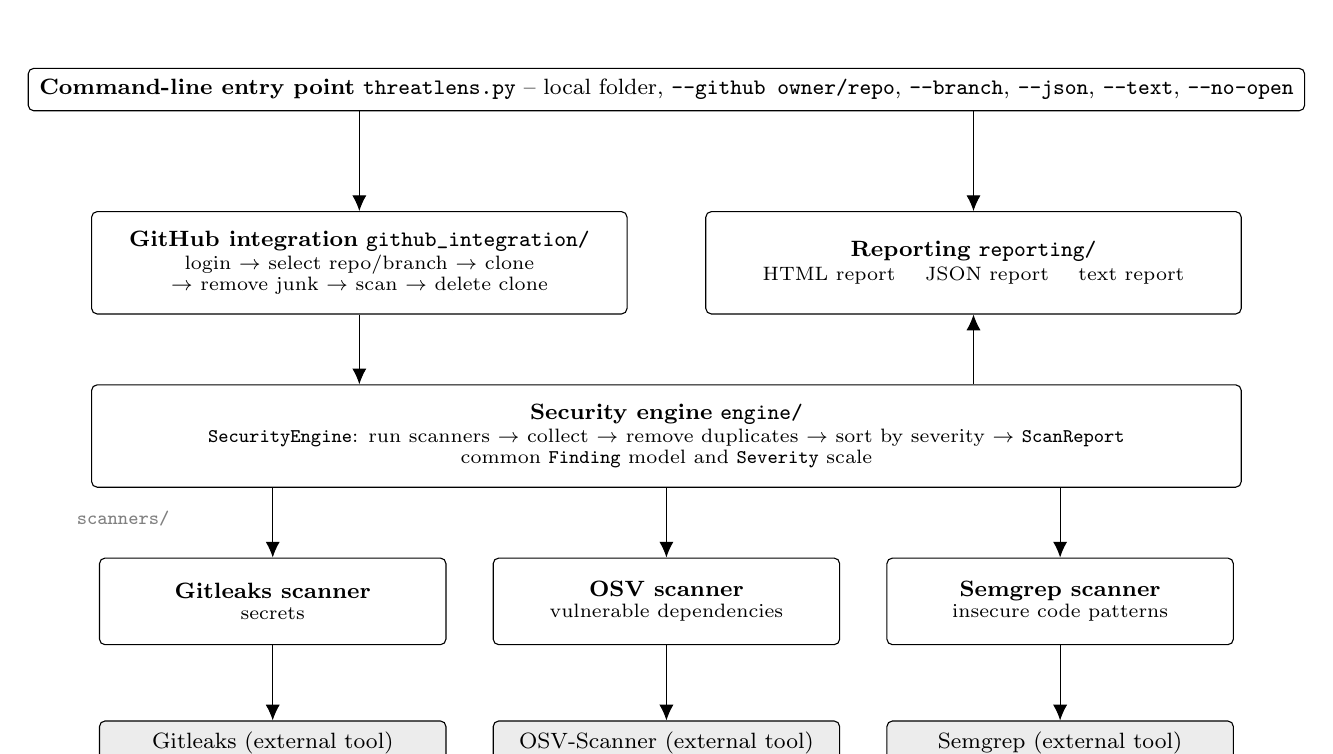
\begin{tikzpicture}[x=1cm,y=1cm]
  \node[lyr,minimum width=14.6cm] (cli) at (0,0) {\textbf{Command-line entry point} \code{threatlens.py} -- local folder, \code{--github owner/repo}, \code{--branch}, \code{--json}, \code{--text}, \code{--no-open}};
  \node[lyr,minimum width=6.8cm,minimum height=1.3cm] (gh) at (-3.9,-2.2) {\textbf{GitHub integration} \code{github_integration/}\\[-1pt]\scriptsize login $\rightarrow$ select repo/branch $\rightarrow$ clone\\[-2pt]\scriptsize $\rightarrow$ remove junk $\rightarrow$ scan $\rightarrow$ delete clone};
  \node[lyr,minimum width=6.8cm,minimum height=1.3cm] (rep) at (3.9,-2.2) {\textbf{Reporting} \code{reporting/}\\[-1pt]\scriptsize HTML report \quad JSON report \quad text report};
  \node[lyr,minimum width=14.6cm,minimum height=1.3cm] (eng) at (0,-4.4) {\textbf{Security engine} \code{engine/}\\[-1pt]\scriptsize \code{SecurityEngine}: run scanners $\rightarrow$ collect $\rightarrow$ remove duplicates $\rightarrow$ sort by severity $\rightarrow$ \code{ScanReport}\\[-2pt]\scriptsize common \code{Finding} model and \code{Severity} scale};
  \node[lyr,minimum width=4.4cm,minimum height=1.1cm] (s1) at (-5.0,-6.5) {\textbf{Gitleaks scanner}\\[-2pt]\scriptsize secrets};
  \node[lyr,minimum width=4.4cm,minimum height=1.1cm] (s2) at (0,-6.5) {\textbf{OSV scanner}\\[-2pt]\scriptsize vulnerable dependencies};
  \node[lyr,minimum width=4.4cm,minimum height=1.1cm] (s3) at (5.0,-6.5) {\textbf{Semgrep scanner}\\[-2pt]\scriptsize insecure code patterns};
  \node[font=\scriptsize,gray] at (-6.9,-5.45) {\code{scanners/}};
  \node[lyr,minimum width=4.4cm,fill=gray!15] (t1) at (-5.0,-8.3) {Gitleaks (external tool)};
  \node[lyr,minimum width=4.4cm,fill=gray!15] (t2) at (0,-8.3) {OSV-Scanner (external tool)};
  \node[lyr,minimum width=4.4cm,fill=gray!15] (t3) at (5.0,-8.3) {Semgrep (external tool)};
  \draw[flow] (cli.south -| gh) -- (gh);
  \draw[flow] (cli.south -| rep) -- (rep);
  \draw[flow] (gh.south) -- (gh |- eng.north);
  \draw[flow] (eng.north -| rep) -- (rep.south);
  \draw[flow] (eng.south -| s1) -- (s1);
  \draw[flow] (eng.south -| s2) -- (s2);
  \draw[flow] (eng.south -| s3) -- (s3);
  \draw[flow] (s1) -- (t1);
  \draw[flow] (s2) -- (t2);
  \draw[flow] (s3) -- (t3);
\end{tikzpicture}}
\caption{Layered architecture of the ThreatLens prototype}
\label{fig:arch}
\end{figure}

\subsection{Project Structure}

The source code of the prototype lives in the folder \code{project a}:

\begin{lstlisting}[language={},caption={Folder structure of the prototype},label={lst:tree}]
project a/
|-- threatlens.py              main command-line entry point
|-- engine/
|   |-- finding.py             Finding dataclass and Severity enum
|   `-- security_engine.py     SecurityEngine, ScannerResult, ScanReport
|-- scanners/
|   |-- gitleaks_scanner.py    secrets
|   |-- osv_scanner.py         vulnerable dependencies
|   `-- semgrep_scanner.py     insecure code patterns
|-- reporting/
|   |-- report_generator.py    plain-text report
|   |-- html_report.py         HTML report
|   `-- json_report.py         JSON report (contract for the extension)
|-- github_integration/
|   |-- client.py              token login
|   |-- repos.py, repo_selector.py, branches.py
|   |-- cloner.py              shallow clone
|   |-- cleanup.py             guaranteed deletion of clones
|   |-- repo_scanner.py        junk removal + scan + relative paths
|   `-- pipeline.py            scan_github_repo(): the whole flow
|-- test-repo/                 controlled repo: fake secrets, old libraries
|-- tests/
|-- run_phase1.py, run_phase5.py, run_stage2.py   per-stage demos
|-- requirements.txt
`-- .gitignore
\end{lstlisting}

\subsection{The Common Finding Model}

Gitleaks, OSV-Scanner and Semgrep each describe problems in a different way. To combine them, every result is converted into one \code{Finding} object (a Python dataclass).

\begin{table}[H]
\centering
\caption{Fields of the \code{Finding} class}
\label{tab:finding}
\begin{tabularx}{\textwidth}{@{}p{3.4cm}p{3.2cm}X@{}}
\toprule
\textbf{Field} & \textbf{Type} & \textbf{Meaning} \\
\midrule
\code{tool} & text & Gitleaks, OSV-Scanner or Semgrep \\
\code{rule} & text & Rule or vulnerability id, e.g. \code{github-pat}, \code{CVE-2022-22817} \\
\code{category} & text & Secret, Dependency Vulnerability, Code Security, etc. \\
\code{severity} & \code{Severity} & CRITICAL, HIGH, MEDIUM, LOW or INFO \\
\code{file}, \code{start_line}, \code{end_line}, \code{start_column}, \code{end_column} & text, integers & Where the problem is \\
\code{description} & text & What is wrong? \\
\code{risk} & text & Why is it dangerous? \\
\code{recommendation} & text & How should it be fixed? \\
\code{reference} & text & Link to a CVE page or rule documentation \\
\code{fingerprint} & text & Unique id used for duplicate removal \\
\bottomrule
\end{tabularx}
\end{table}

\begin{table}[H]
\centering
\caption{Severity scale}
\label{tab:severity}
\begin{tabularx}{\textwidth}{@{}lX@{}}
\toprule
\textbf{Severity} & \textbf{Meaning} \\
\midrule
CRITICAL & Production secret exposed, private key, or CVSS score 9.0 or higher \\
HIGH & API key or access token, CVSS 7.0--8.9 \\
MEDIUM & Generic credential pattern, CVSS 4.0--6.9 \\
LOW & Informational code smell, CVSS below 4.0 \\
INFO & Best-practice suggestion with no immediate risk \\
\bottomrule
\end{tabularx}
\end{table}

\subsection{Scanner Wrappers}

Each wrapper has one public method, \code{scan(repo_path)}, which returns a list of \code{Finding} objects. Because the engine only needs this method, a new scanner can be added without changing the engine.

\begin{longtable}{@{}p{2.0cm}p{2.3cm}p{5.0cm}p{4.7cm}@{}}
\caption{The three scanner wrappers}\label{tab:scanners}\\
\toprule
\textbf{Wrapper} & \textbf{Detects} & \textbf{Command used} & \textbf{Severity rule} \\
\midrule
\endfirsthead
\toprule
\textbf{Wrapper} & \textbf{Detects} & \textbf{Command used} & \textbf{Severity rule} \\
\midrule
\endhead
Gitleaks & Hardcoded secrets & \code{gitleaks} \code{detect} \code{--source} \code{<path>} \code{--report-format} \code{json} \code{--report-path} \code{<file>}; \code{--no-git} is added when the folder has no \code{.git} & Lookup table by rule id: private keys CRITICAL; specific tokens (GitHub, AWS, Slack, Stripe, \dots) HIGH; generic passwords and keys MEDIUM \\
OSV-Scanner & Dependencies with known vulnerabilities & \code{osv-scanner} \code{scan} \code{--format} \code{json} \code{--recursive} \code{<path>} & CVSS score: 9.0 or more CRITICAL, 7.0 or more HIGH, 4.0 or more MEDIUM, otherwise LOW \\
Semgrep & Insecure code patterns & \code{semgrep} \code{scan} \code{--config} \code{auto} \code{--json} \code{--quiet} \code{--no-git-ignore} \code{<path>} & Semgrep level: ERROR $\rightarrow$ HIGH, WARNING $\rightarrow$ MEDIUM, INFO $\rightarrow$ LOW, NOTE $\rightarrow$ INFO \\
\bottomrule
\end{longtable}

Two details matter in practice. First, Gitleaks, OSV-Scanner and Semgrep return exit code 1 when they \emph{find} something; this is not an error, so the wrappers accept exit codes 0 and 1 and treat anything else as a real failure. Second, each wrapper writes the plain-language \emph{description}, \emph{risk} and \emph{recommendation} text itself, so that the final report reads the same whichever tool produced the finding.

\subsection{SecurityEngine}

The \code{SecurityEngine} is the central coordinator. Callers only need to know about the engine, not about which scanners exist or how they work.

\begin{enumerate}
    \item \textbf{Register} scanners with \code{add_scanner(name, scanner)}. The engine checks that the object really has a \code{scan} method (a \code{Scanner} protocol).
    \item \textbf{Run} every scanner. Each run is wrapped in a \code{try/except}, so a scanner that crashes is recorded as failed (with its error message) and the others continue.
    \item \textbf{Collect} the findings of all successful scanners.
    \item \textbf{Remove duplicates} using the \code{fingerprint} field: the first finding with a given fingerprint is kept.
    \item \textbf{Sort} by severity (CRITICAL first), then by file and line.
    \item \textbf{Return} a \code{ScanReport} holding the findings, the per-scanner results, the total, a count per severity and the list of failed scanners.
\end{enumerate}

\subsection{Reporting}

\begin{itemize}
    \item \textbf{HTML report (default):} one self-contained page with a summary table, a list of all findings and, for each finding, the sections \emph{What is wrong}, \emph{Why it matters}, \emph{How to fix} and \emph{Reference}. Every value from the scanned repository (file names, messages) is HTML-escaped, because it comes from an unknown source. The page has print rules so that \emph{Print $\rightarrow$ Save as PDF} gives a clean PDF.
    \item \textbf{JSON report (\code{--json}):} one JSON object on standard output with \code{schema_version}, \code{status}, \code{summary}, \code{total}, the status of each scanner and the list of findings with paths relative to the scanned folder. It is the contract with the future VS Code extension. If the scan cannot run, a JSON error object with \code{status: error} is printed instead.
    \item \textbf{Text report (\code{--text}):} a full report printed in the terminal.
\end{itemize}

\subsection{GitHub Integration}

The whole GitHub scan is available as one function, \code{scan_github_repo(repo, branch)}. It never asks the user anything and never prints, so a server (Stage~5) can call it safely; interactive questions such as ``which branch?'' are handled only in the command-line program.

\begin{enumerate}
    \item \textbf{Log in} (\code{client.py}): a fine-grained personal access token is read from the \code{GITHUB_TOKEN} environment variable or a \code{.env} file, and one cheap API call proves that it works. Only this file knows how login is done, so a later switch to a GitHub App changes one file.
    \item \textbf{Select the repository} (\code{repo_selector.py}): accepts \code{owner/repo} or common GitHub URL forms, checks the name format, asks GitHub for the repository and refuses empty repositories and those above 500\,MB.
    \item \textbf{Select the branch} (\code{branches.py}): lists branches (default branch first) and, in interactive use, shows a numbered menu.
    \item \textbf{Clone} (\code{cloner.py}): \code{git clone --depth 1 --single-branch} into a unique temporary folder; the exact commit id is recorded.
    \item \textbf{Remove junk} (\code{repo_scanner.py}): folders such as \code{node_modules}, \code{site-packages}, caches and any Python virtual environment (detected by its \code{pyvenv.cfg} file) are deleted from the \emph{copy} only, to avoid slow scans and hundreds of false alarms from other people's code.
    \item \textbf{Scan:} the same \code{SecurityEngine} is used, unchanged; absolute file paths are converted to repository-relative paths.
    \item \textbf{Always delete the clone} (\code{cleanup.py}): the clone is created in a \code{with} block (\code{temporary_clone}), so it is deleted on success, on error and on Ctrl+C. Clones left behind by a hard shutdown are removed on the next run if they are older than 24 hours.
\end{enumerate}

\subsection{Security Decisions Built into the Design}

\begin{table}[H]
\centering
\caption{Security-related design decisions}
\label{tab:security}
\begin{tabularx}{\textwidth}{@{}p{4.3cm}X@{}}
\toprule
\textbf{Decision} & \textbf{Reason} \\
\midrule
Redact secrets (keep at most 4 characters, e.g.\ \code{ghp_***}) & A security tool must not become a new place where secrets leak. \\
Token sent in an HTTP header through environment variables & The token never appears in the clone URL, in \code{.git/config} or on the command line, and error messages have it masked. \\
Delete only inside the clone folder & A bug that passes the wrong path can never delete the user's own files (\code{remove_tree} refuses any path that is not strictly inside the clone folder). \\
Suggest fixes, never apply them & Automatic changes could break working code; a person decides. \\
HTML-escape all scanned values & A file named like a script tag must not run in the reader's browser. \\
\bottomrule
\end{tabularx}
\end{table}
% =====================================================================
%                          6. UML DIAGRAMS
% =====================================================================
\section{UML Diagrams}

This section models the prototype with UML diagrams, following the notation taught in the course: the use case diagram with its use case templates, the class diagram, the sequence diagram, the activity diagram, the component diagram and the deployment diagram. The diagrams describe what is implemented in the prototype (Module~1, stages 1--4). The relationships are written as \guillemotleft includes\guillemotright{} and \guillemotleft extends\guillemotright{}, and merges in the activity diagram use merge diamonds (UML~2).

% ---------------------------------------------------------------------
\subsection{Use Case Diagram}

\textbf{Actors.} The \emph{Developer} is the primary actor: the person who runs ThreatLens. \emph{GitHub} and the \emph{Scanner tools} (Gitleaks, OSV-Scanner, Semgrep) are external systems that ThreatLens uses; they are outside the system boundary.

\begin{table}[H]
\centering
\caption{Use cases of the prototype}
\label{tab:usecases}
\begin{tabularx}{\textwidth}{@{}p{1.1cm}p{4.2cm}X@{}}
\toprule
\textbf{ID} & \textbf{Use case} & \textbf{Description} \\
\midrule
UC1 & Scan Local Folder & Scan a folder on the computer with all three scanners and produce a report. \\
UC2 & Scan GitHub Repository & Scan one branch of a GitHub repository in a temporary clone and produce a report. \\
UC3 & Run Security Scanners & Run Gitleaks, OSV-Scanner and Semgrep, remove duplicates and sort the findings (included by UC1 and UC2). \\
UC4 & Authenticate with GitHub & Log in with the access token and check that it works (included by UC2 and UC6). \\
UC5 & Clone Repository & Take a temporary shallow clone, remove junk folders, delete the clone after the scan (included by UC2). \\
UC6 & List Branches & Show the branches of a repository. \\
UC7 & Select Branch & Let the user choose a branch when none was given (extends UC2). \\
UC8 & View Security Report & Read the report as HTML, JSON or text. \\
\bottomrule
\end{tabularx}
\end{table}

\begin{figure}[H]
\centering
\resizebox{\textwidth}{!}{%
\begin{tikzpicture}[x=1cm,y=1cm]
  % system boundary
  \draw[sysbox] (2.4,0.3) rectangle (14.4,10.6);
  \node[anchor=north west,font=\footnotesize\bfseries] at (2.55,10.55) {ThreatLens (prototype)};

  % actors
  \stickman{0.8}{5.2}{dev}{Developer}
  \stickman{16.3}{4.8}{gh}{GitHub\\(external system)}
  \stickman{16.3}{9.2}{tools}{Scanner tools\\(Gitleaks, OSV-Scanner,\\Semgrep)}

  % use cases
  \node[uc] (A) at (4.4,9.2)  {UC1\\Scan Local Folder};
  \node[uc] (B) at (4.4,6.3)  {UC2\\Scan GitHub Repository};
  \node[uc] (V) at (4.4,1.5)  {UC8\\View Security Report};
  \node[uc] (E) at (8.6,9.2)  {UC3\\Run Security Scanners};
  \node[uc] (G) at (8.6,7.0)  {UC5\\Clone Repository};
  \node[uc] (H) at (8.6,4.4)  {UC7\\Select Branch};
  \node[uc] (C) at (8.6,2.0)  {UC6\\List Branches};
  \node[uc] (F) at (12.5,4.8) {UC4\\Authenticate with GitHub};

  % associations
  \draw (dev) -- (A.west);
  \draw (dev) -- (B.west);
  \draw (dev) -- (V.west);
  \draw (dev) -- (C.south west);
  \draw (gh) -- (F.east);
  \draw (gh) -- (G.east);
  \draw (gh) -- (C.east);
  \draw (tools) -- (E.east);

  % include / extend
  \draw[dep] (A) -- node[midway,fill=white,inner sep=1pt,font=\tiny] {\guillemotleft includes\guillemotright} (E);
  \draw[dep] (B) -- node[pos=0.45,fill=white,inner sep=1pt,font=\tiny] {\guillemotleft includes\guillemotright} (E);
  \draw[dep] (B) -- node[midway,fill=white,inner sep=1pt,font=\tiny] {\guillemotleft includes\guillemotright} (G);
  \draw[dep] (B) -- node[pos=0.55,fill=white,inner sep=1pt,font=\tiny] {\guillemotleft includes\guillemotright} (F);
  \draw[dep] (C) -- node[midway,fill=white,inner sep=1pt,font=\tiny] {\guillemotleft includes\guillemotright} (F);
  \draw[dep] (H) -- node[midway,fill=white,inner sep=1pt,font=\tiny] {\guillemotleft extends\guillemotright} (B);
\end{tikzpicture}}
\caption{Use case diagram of the ThreatLens prototype}
\label{fig:usecase}
\end{figure}

% ---------------------------------------------------------------------
\subsection{Use Case Templates}

\textbf{Typical flow notation:} AA = actor action, SR = system response.

\begin{longtable}{|p{3.8cm}|p{10.8cm}|}
\caption{Use case template: UC1 Scan Local Folder}\label{tab:uc1}\\
\hline
\textbf{1. Use Case Title} & Scan Local Folder \\ \hline
\textbf{2. Abbreviated Title} & Local Scan \\ \hline
\textbf{3. Use Case Id} & UC1 \\ \hline
\textbf{4. Actors} & Developer (primary); Scanner tools (external systems) \\ \hline
\textbf{5. Description} & The developer scans a folder on his or her own computer. ThreatLens runs all three scanners and gives one report with plain-language explanations. \\ \hline
\textbf{5.1 Pre-conditions} & The folder exists. Gitleaks, OSV-Scanner and Semgrep are installed. \\ \hline
\textbf{5.2 Task Sequence (normal flow)} &
1.\,(AA) The developer runs \code{python threatlens.py ./folder}.\newline
2.\,(SR) The system checks that the folder exists.\newline
3.\,(SR) The system runs Gitleaks, OSV-Scanner and Semgrep one after another.\newline
4.\,(SR) The system removes duplicate findings and sorts them by severity.\newline
5.\,(SR) The system writes the HTML report, opens it in the browser and prints a short summary.\newline
6.\,(AA) The developer reads the report and fixes the problems. \\ \hline
\textbf{5.3 Alternate flow} & 5a. With \code{--json} the system prints one JSON object; with \code{--text} it prints the full text report in the terminal; with \code{--no-open} the browser is not opened. \\ \hline
\textbf{5.4 Exceptional flow} & 2a. The folder does not exist: the system shows an error and ends with exit code 2.\newline
3a. A scanner fails or is not installed: the failure is recorded, the other scanners still run, and the report says that results are incomplete. \\ \hline
\textbf{5.5 Post-conditions} & A report is available. The scanned code is unchanged. Exit code is 0 (no HIGH/CRITICAL issues) or 1 (HIGH or CRITICAL issues found). \\ \hline
\textbf{6. Modification History} & 13-Oct-2026 \\ \hline
\textbf{7. Author} & ThreatLens team, Group 3C52 \\ \hline
\end{longtable}

\begin{longtable}{|p{3.8cm}|p{10.8cm}|}
\caption{Use case template: UC2 Scan GitHub Repository}\label{tab:uc2}\\
\hline
\textbf{1. Use Case Title} & Scan GitHub Repository \\ \hline
\textbf{2. Abbreviated Title} & GitHub Scan \\ \hline
\textbf{3. Use Case Id} & UC2 \\ \hline
\textbf{4. Actors} & Developer (primary); GitHub and Scanner tools (external systems) \\ \hline
\textbf{5. Description} & The developer scans one branch of a GitHub repository without downloading it manually. ThreatLens clones it temporarily, scans it, deletes the clone and reports the findings. \\ \hline
\textbf{5.1 Pre-conditions} & A valid GitHub access token is in \code{GITHUB_TOKEN} or in the \code{.env} file. \code{git} and the three scanners are installed. The token can access the repository. \\ \hline
\textbf{5.2 Task Sequence (normal flow)} &
1.\,(AA) The developer runs \code{python threatlens.py --github owner/repo}.\newline
2.\,(SR) The system reads the token, logs in to GitHub and shows the user name.\newline
3.\,(SR) The system looks up the repository and checks that it is not empty and not larger than 500\,MB.\newline
4.\,(SR) The system lists the branches (default first) and asks which one to scan.\newline
5.\,(AA) The developer chooses a branch or presses Enter for the default branch.\newline
6.\,(SR) The system makes a shallow clone of the branch in a unique temporary folder and records the commit id.\newline
7.\,(SR) The system removes junk folders (installed libraries, virtual environments, caches) from the copy.\newline
8.\,(SR) The system runs the three scanners, removes duplicates, sorts by severity and makes file paths relative to the repository.\newline
9.\,(SR) The system deletes the temporary clone.\newline
10.\,(SR) The system writes the report (repository, branch and commit are shown) and prints a short summary.\newline
11.\,(AA) The developer reads the report and fixes the problems. \\ \hline
\textbf{5.3 Alternate flow} & 4a. If \code{--branch name} is given, or the run is not interactive, or \code{--json} is used, no question is asked and the given or default branch is scanned.\newline
10a. \code{--json}, \code{--text} and \code{--no-open} change the output as in UC1. \\ \hline
\textbf{5.4 Exceptional flow} & 2a. The token is missing, mistyped, expired or revoked: error message, exit code 2.\newline
3a. The repository is not found, the token has no access, or the repository is empty or too large: error message, exit code 2.\newline
6a. The branch does not exist, \code{git} is missing, or cloning takes longer than 5 minutes: error message, exit code 2.\newline
8a. A scanner fails: the others continue and the report marks the results as incomplete.\newline
*.\ If the user presses Ctrl+C, the temporary clone is still deleted. \\ \hline
\textbf{5.5 Post-conditions} & A report is available. The temporary clone is deleted. The repository on GitHub is unchanged. Exit code is 0, 1 or 2 as above. \\ \hline
\textbf{6. Modification History} & 13-Oct-2026 \\ \hline
\textbf{7. Author} & ThreatLens team, Group 3C52 \\ \hline
\end{longtable}

% ---------------------------------------------------------------------
\subsection{Class Diagram}

Figure~\ref{fig:class1} shows the core of the engine. \code{SecurityEngine} is made of one or more scanners that follow the \code{Scanner} interface; the three wrappers realise that interface. The engine produces a \code{ScanReport}, which is composed of \code{Finding} objects and \code{ScannerResult} objects. Every scanner wrapper creates \code{Finding} objects, and each \code{Finding} has a \code{Severity}.

\begin{figure}[H]
\centering
\resizebox{\textwidth}{!}{%
\begin{tikzpicture}[x=1cm,y=1cm,
  cls3/.style={cls,text width=3.2cm}]
  \node[cls] (Eng) at (2.3,0) {\cname{SecurityEngine}
    \nodepart{second}-repo\_path: str\\-\_scanners: list[(str, Scanner)]
    \nodepart{third}+add\_scanner(name, scanner)\\+scan(): ScanReport\\-\_run\_scanner(name, scanner)\\-\_deduplicate(findings)\\-\_sort\_by\_severity(findings)};

  \node[cls3] (Sc) at (11.2,0) {\cstereo{interface}{Scanner}
    \nodepart{second}\ 
    \nodepart{third}+scan(repo\_path: str):\\\ \ list[Finding]};

  \node[cls3] (Gl) at (7.4,-3.9) {\cname{GitleaksScanner}
    \nodepart{second}-gitleaks\_cmd: str
    \nodepart{third}+scan(repo\_path): list[Finding]};
  \node[cls3] (Os) at (11.2,-3.9) {\cname{OsvScanner}
    \nodepart{second}-osv\_cmd: str
    \nodepart{third}+scan(repo\_path): list[Finding]};
  \node[cls3] (Se) at (15.0,-3.9) {\cname{SemgrepScanner}
    \nodepart{second}-semgrep\_cmd: str\\-config: str
    \nodepart{third}+scan(repo\_path): list[Finding]};

  \node[cls,text width=4.6cm] (Rep) at (2.4,-6.1) {\cname{ScanReport}
    \nodepart{second}+repo\_path: str\\+findings: list[Finding]\\+scanner\_results: list[ScannerResult]
    \nodepart{third}+total: int\\+summary: dict\\+failed\_scanners: list\\+has\_severity(severity): bool};

  \node[cls3] (SR) at (2.3,-11.4) {\cname{ScannerResult}
    \nodepart{second}+scanner\_name: str\\+success: bool\\+findings: list[Finding]\\+error: str
    \nodepart{third}\ };

  \node[cls,text width=4.4cm] (Fi) at (9.6,-10.4) {\cname{Finding}
    \nodepart{second}+tool, rule, category: str\\+severity: Severity\\+file: str\\+start\_line, end\_line: int\\+description, risk: str\\+recommendation: str\\+reference, fingerprint: str
    \nodepart{third}+to\_dict(): dict};

  \node[cls3] (Sv) at (15.4,-10.4) {\cstereo{enumeration}{Severity}
    \nodepart{second}CRITICAL\\HIGH\\MEDIUM\\LOW\\INFO
    \nodepart{third}\ };

  % relationships
  \draw[aggr] (Eng.east) -- node[above,font=\tiny,pos=0.8] {1..*} (Sc.west);
  \draw[real] (Gl.north) -- ++(0,0.8) -| (Sc.south);
  \draw[real] (Os.north) -- (Sc.south);
  \draw[real] (Se.north) -- ++(0,0.8) -| (Sc.south);
  \draw[dep] (Eng.south) -- node[right,font=\tiny] {\guillemotleft creates\guillemotright} (Rep.north);
  \draw[comp] (Rep.south) -- node[right,font=\tiny,pos=0.8] {0..*} (SR.north);
  \draw[comp] (Rep.east) -| node[above,font=\tiny,pos=0.25] {0..*} (Fi.north);
  \draw[assoc] (SR.east) -- node[above,font=\tiny] {0..*} (Fi.west);
  \draw[assoc] (Fi.east) -- node[above,font=\tiny] {severity} (Sv.west);
  \draw[dep] (Os.south) -- node[right,font=\tiny,pos=0.5] {\guillemotleft returns\guillemotright} (Os.south |- Fi.north);
\end{tikzpicture}}
\caption{Class diagram: scanners, engine, report and finding}
\label{fig:class1}
\end{figure}

Figure~\ref{fig:class2} shows the data classes of the GitHub integration. The functions of that package are grouped in modules (\guillemotleft module\guillemotright), not classes: \code{client}, \code{repo_selector}, \code{branches}, \code{cloner}, \code{cleanup}, \code{repo_scanner} and \code{pipeline}. The single function \code{scan_github_repo()} in \code{pipeline} uses the others and returns a \code{GitHubScanResult}.

\begin{figure}[H]
\centering
\resizebox{\textwidth}{!}{%
\begin{tikzpicture}[x=1cm,y=1cm,
  cls3/.style={cls,text width=3.6cm}]
  \node[cls,text width=6.6cm] (Mod) at (3.6,0) {\cstereo{module}{github\_integration}
    \nodepart{second}client: get\_github\_client(), verify\_connection()\\repo\_selector: select\_repo()\\branches: list\_branches(), prompt\_for\_branch()\\cloner: clone\_repo()\\cleanup: temporary\_clone(), remove\_tree(), cleanup\_stale\_clones()\\repo\_scanner: remove\_junk\_dirs(), scan\_cloned\_repo()
    \nodepart{third}pipeline: +scan\_github\_repo(repo, branch, gh, token): GitHubScanResult};

  \node[cls3] (Gs) at (12.0,0.6) {\cname{GitHubScanResult}
    \nodepart{second}+repo: RepoInfo\\+branch: str\\+commit\_sha: str\\+report: ScanReport\\+skipped\_dirs: list[str]
    \nodepart{third}+short\_sha: str};

  \node[cls3] (Ri) at (17.0,3.6) {\cname{RepoInfo}
    \nodepart{second}+full\_name: str\\+private: bool\\+default\_branch: str\\+size\_kb: int\\+language: str\\+clone\_url: str
    \nodepart{third}+from\_github(repo): RepoInfo};

  \node[cls3] (Sr) at (17.0,-2.4) {\cstereo{from engine}{ScanReport}
    \nodepart{second}\ 
    \nodepart{third}\ };

  \node[cls3] (Cr) at (12.0,-4.6) {\cname{ClonedRepo}
    \nodepart{second}+full\_name: str\\+path: Path\\+ref: str\\+commit\_sha: str
    \nodepart{third}\ };

  \draw[dep] (Mod.east) -- node[above,font=\tiny] {\guillemotleft creates\guillemotright} (Gs.west);
  \draw[comp] (Gs.east) -- node[above,font=\tiny,pos=0.3,sloped] {1} (Ri.west);
  \draw[assoc] (Gs.east) -- node[below,font=\tiny,pos=0.3,sloped] {1} (Sr.west);
  \draw[dep] (Mod.south east) |- node[above,font=\tiny,pos=0.75] {\guillemotleft uses\guillemotright} (Cr.west);
\end{tikzpicture}}
\caption{Class diagram: GitHub integration}
\label{fig:class2}
\end{figure}

% ---------------------------------------------------------------------
\subsection{Sequence Diagram}

Figure~\ref{fig:seq} shows the objects and messages for the main scenario, scanning a GitHub repository (UC2). Solid arrows are calls, dashed arrows are returns. The branch question (messages 4 and 5) is asked only in interactive use.

\begin{figure}[H]
\centering
\resizebox{\textwidth}{!}{%
\begin{tikzpicture}[x=1cm,y=1cm]
  \newcommand{\selfmsg}[3]{\draw[msg] (#1+0.1,#2) -- ++(0.6,0) -- ++(0,-0.4) -- (#1+0.1,#2-0.4); \node[font=\tiny,anchor=west] at (#1+0.75,#2-0.2) {#3};}
  % object boxes and lifelines
  \foreach \n/\x/\l in {dev/0/Developer, cli/3/{:CLI\\(threatlens.py)}, gh/6/{:GitHub\\(API / remote)}, pl/9/{:Pipeline\\(pipeline.py)}, en/12/{:SecurityEngine}, sc/15/{:Scanners\\(Gitleaks, OSV,\\Semgrep)}} {
    \node[draw,align=center,font=\scriptsize,minimum width=2.2cm,minimum height=0.9cm,fill=white] (\n) at (\x,0) {\l};
    \draw[dashed] (\x,-0.55) -- (\x,-16.2);
  }
  % activation bars
  \foreach \x/\a/\b in {0/-1.0/-1.5, 0/-3.2/-4.3, 0/-14.9/-15.3, 3/-1.0/-15.2, 6/-1.8/-2.8, 6/-5.5/-6.4, 6/-6.9/-7.9, 9/-4.7/-13.9, 12/-9.1/-12.3, 15/-9.9/-10.9} {
    \draw[fill=white] (\x-0.1,\a) rectangle (\x+0.1,\b);
  }
  % messages
  \draw[msg] (0.1,-1.2) -- node[above,font=\tiny] {1: run {-}{-}github owner/repo} (2.9,-1.2);
  \draw[msg] (3.1,-2.0) -- node[above,font=\tiny] {2: verify token} (5.9,-2.0);
  \draw[ret] (5.9,-2.7) -- node[above,font=\tiny] {3: user name} (3.1,-2.7);
  \draw[ret] (2.9,-3.4) -- node[above,font=\tiny] {4: which branch?} (0.1,-3.4);
  \draw[msg] (0.1,-4.1) -- node[above,font=\tiny] {5: branch} (2.9,-4.1);
  \draw[msg] (3.1,-4.9) -- node[above,font=\tiny] {6: scan\_github\_repo(repo, branch)} (8.9,-4.9);
  \draw[msg] (9.1,-5.7) -- node[above,font=\tiny] {7: select\_repo} (5.9,-5.7);
  \draw[ret] (5.9,-6.3) -- node[above,font=\tiny] {8: repo info} (9.1,-6.3);
  \draw[msg] (9.1,-7.1) -- node[above,font=\tiny] {9: git clone {-}{-}depth 1} (5.9,-7.1);
  \draw[ret] (5.9,-7.7) -- node[above,font=\tiny] {10: snapshot, commit id} (9.1,-7.7);
  \selfmsg{9}{-8.4}{11: remove junk folders}
  \draw[msg] (9.1,-9.3) -- node[above,font=\tiny] {12: scan()} (11.9,-9.3);
  \draw[msg] (12.1,-10.1) -- node[above,font=\tiny] {13: scan(repo\_path)} (14.9,-10.1);
  \draw[ret] (14.9,-10.7) -- node[above,font=\tiny] {14: findings} (12.1,-10.7);
  \selfmsg{12}{-11.3}{15: deduplicate, sort}
  \draw[ret] (11.9,-12.2) -- node[above,font=\tiny] {16: ScanReport} (9.1,-12.2);
  \selfmsg{9}{-12.8}{17: delete temporary clone}
  \draw[ret] (8.9,-13.8) -- node[above,font=\tiny] {18: GitHubScanResult} (3.1,-13.8);
  \selfmsg{3}{-14.3}{19: write report}
  \draw[ret] (2.9,-15.1) -- node[above,font=\tiny] {20: summary, report path} (0.1,-15.1);
\end{tikzpicture}}
\caption{Sequence diagram: scanning a GitHub repository (UC2)}
\label{fig:seq}
\end{figure}

% ---------------------------------------------------------------------
\subsection{Activity Diagram}

Figure~\ref{fig:activity} shows the overall flow of one run, with swimlanes for the Developer, ThreatLens and GitHub. The scanners run one after another; a failing scanner is recorded and does not stop the rest. Any failure before scanning (folder missing, bad token, repository not found, clone error) ends the run with an error message and exit code 2.

\begin{figure}[H]
\centering
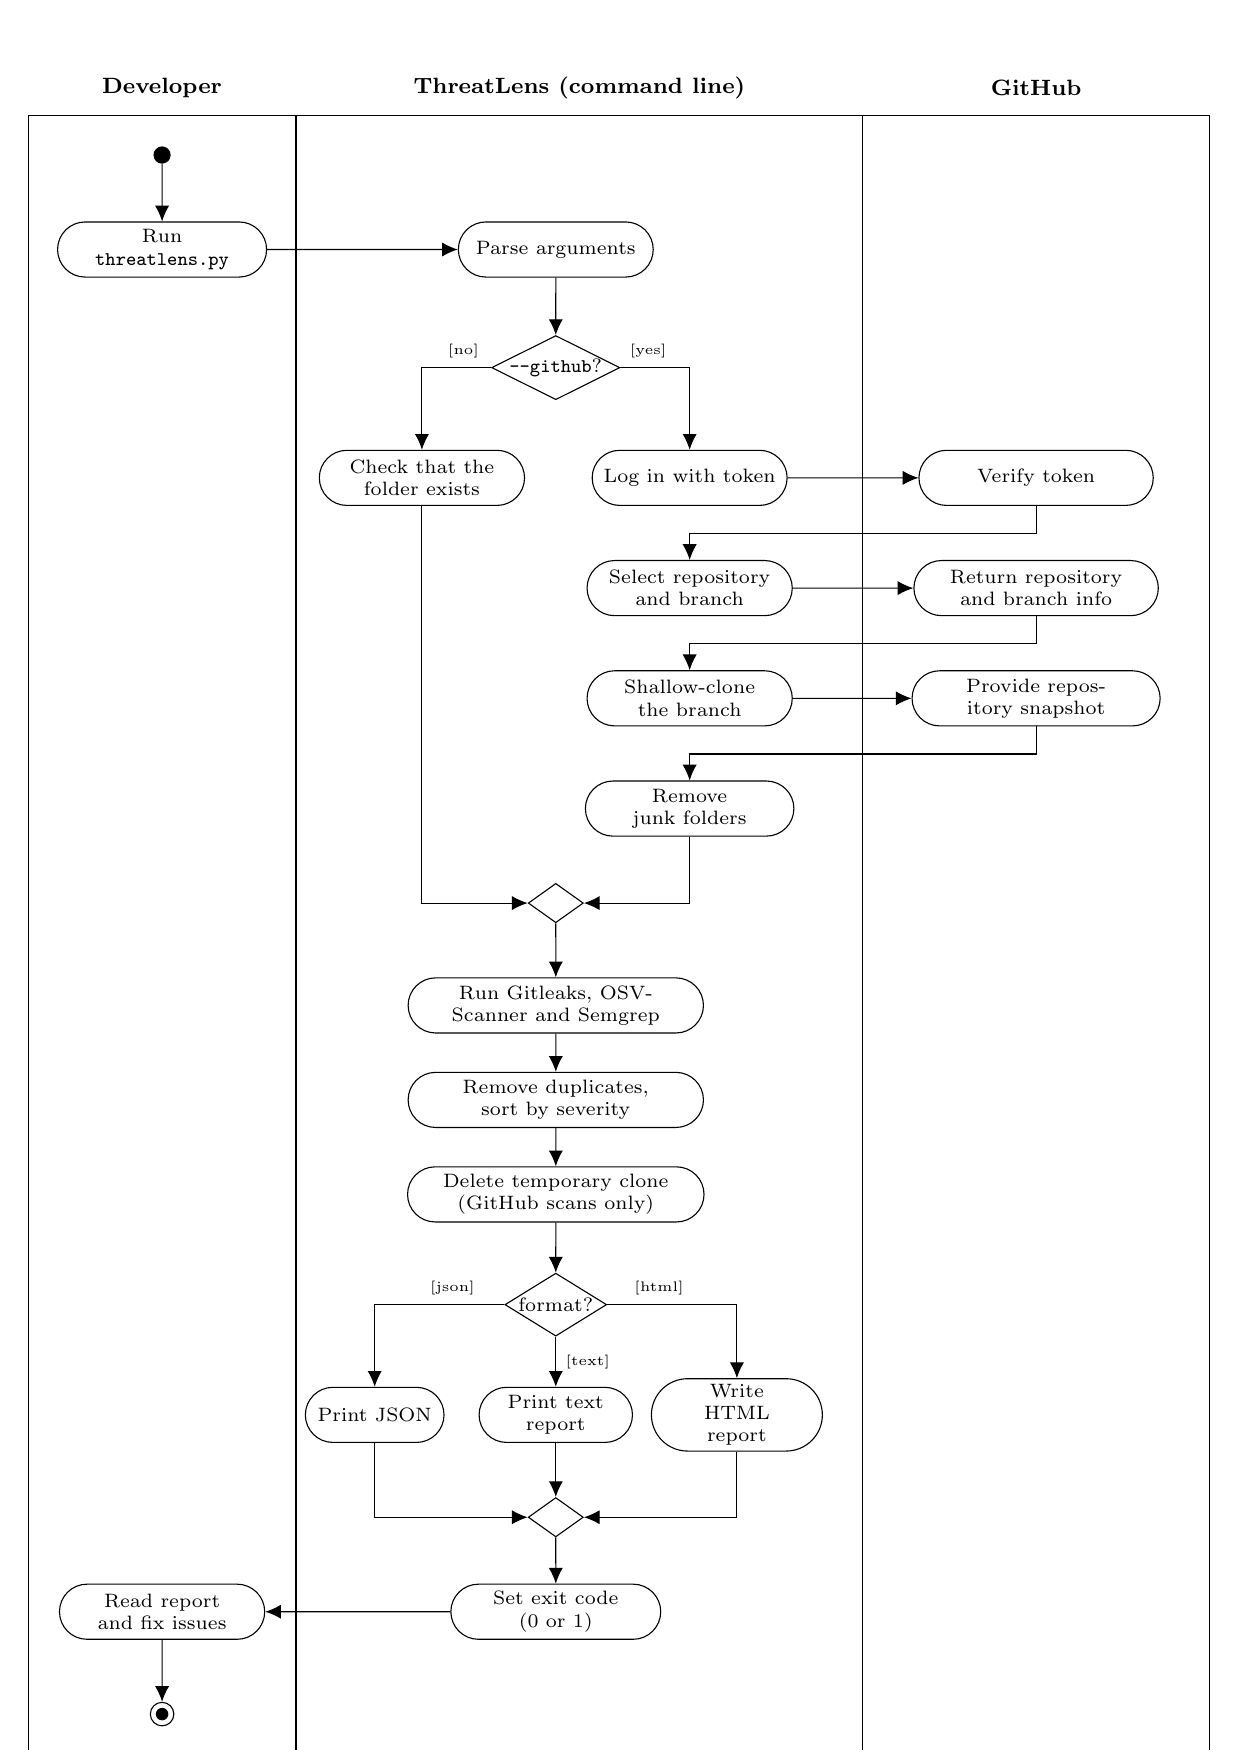
\begin{tikzpicture}[x=1cm,y=1cm]
  % lanes
  \draw (0,0.5) rectangle (3.4,-20.4);
  \draw (3.4,0.5) rectangle (10.6,-20.4);
  \draw (10.6,0.5) rectangle (15.0,-20.4);
  \node[font=\footnotesize\bfseries] at (1.7,0.85) {Developer};
  \node[font=\footnotesize\bfseries] at (7.0,0.85) {ThreatLens (command line)};
  \node[font=\footnotesize\bfseries] at (12.8,0.85) {GitHub};

  \node[circle,fill=black,inner sep=2.2pt] (st) at (1.7,0) {};
  \node[act] (D1) at (1.7,-1.2) {Run \code{threatlens.py}};
  \node[act] (T1) at (6.7,-1.2) {Parse arguments};
  \node[dec] (d1) at (6.7,-2.7) {\code{--github}?};
  \node[act] (L1) at (5.0,-4.1) {Check that the folder exists};
  \node[act] (G1) at (8.4,-4.1) {Log in with token};
  \node[act,text width=2.8cm] (V1) at (12.8,-4.1) {Verify token};
  \node[act] (G2) at (8.4,-5.5) {Select repository and branch};
  \node[act,text width=2.8cm] (R1) at (12.8,-5.5) {Return repository and branch info};
  \node[act] (G3) at (8.4,-6.9) {Shallow-clone the branch};
  \node[act,text width=2.8cm] (C1) at (12.8,-6.9) {Provide repository snapshot};
  \node[act] (G4) at (8.4,-8.3) {Remove junk folders};
  \node[mrg] (m1) at (6.7,-9.5) {};
  \node[act,text width=3.4cm] (S1) at (6.7,-10.8) {Run Gitleaks, OSV-Scanner and Semgrep};
  \node[act,text width=3.4cm] (S2) at (6.7,-12.0) {Remove duplicates, sort by severity};
  \node[act,text width=3.4cm] (S3) at (6.7,-13.2) {Delete temporary clone (GitHub scans only)};
  \node[dec] (d3) at (6.7,-14.6) {format?};
  \node[act,text width=1.6cm] (O1) at (4.4,-16.0) {Print JSON};
  \node[act,text width=1.6cm] (O2) at (6.7,-16.0) {Print text report};
  \node[act,text width=1.6cm] (O3) at (9.0,-16.0) {Write HTML report};
  \node[mrg] (m2) at (6.7,-17.3) {};
  \node[act] (X1) at (6.7,-18.5) {Set exit code (0 or 1)};
  \node[act] (D2) at (1.7,-18.5) {Read report and fix issues};
  \node[circle,draw,inner sep=3pt] (en) at (1.7,-19.8) {};
  \node[circle,fill=black,inner sep=1.6pt] at (en) {};

  \draw[flow] (st) -- (D1);
  \draw[flow] (D1) -- (T1);
  \draw[flow] (T1) -- (d1);
  \draw[flow] (d1.west) -| node[above,font=\tiny,pos=0.2] {[no]} (L1.north);
  \draw[flow] (d1.east) -| node[above,font=\tiny,pos=0.2] {[yes]} (G1.north);
  \draw[flow] (G1) -- (V1);
  \draw[flow] (V1.south) -- ++(0,-0.35) -| (G2.north);
  \draw[flow] (G2) -- (R1);
  \draw[flow] (R1.south) -- ++(0,-0.35) -| (G3.north);
  \draw[flow] (G3) -- (C1);
  \draw[flow] (C1.south) -- ++(0,-0.35) -| (G4.north);
  \draw[flow] (L1.south) |- (m1.west);
  \draw[flow] (G4.south) |- (m1.east);
  \draw[flow] (m1) -- (S1);
  \draw[flow] (S1) -- (S2);
  \draw[flow] (S2) -- (S3);
  \draw[flow] (S3) -- (d3);
  \draw[flow] (d3.west) -| node[above,font=\tiny,pos=0.2] {[json]} (O1.north);
  \draw[flow] (d3.south) -- node[right,font=\tiny] {[text]} (O2.north);
  \draw[flow] (d3.east) -| node[above,font=\tiny,pos=0.2] {[html]} (O3.north);
  \draw[flow] (O1.south) |- (m2.west);
  \draw[flow] (O2.south) -- (m2.north);
  \draw[flow] (O3.south) |- (m2.east);
  \draw[flow] (m2) -- (X1);
  \draw[flow] (X1) -- (D2);
  \draw[flow] (D2) -- (en);
\end{tikzpicture}
\caption{Activity diagram with swimlanes: one ThreatLens run}
\label{fig:activity}
\end{figure}

% ---------------------------------------------------------------------
\subsection{Component Diagram}

The component diagram shows the physical structure of the implementation: the packages of ThreatLens, the external tools and libraries they depend on, and the artifacts they produce.

\begin{figure}[H]
\centering
\resizebox{\textwidth}{!}{%
\begin{tikzpicture}[x=1cm,y=1cm,
  comp/.style={draw,minimum height=1.0cm,font=\scriptsize,align=center,fill=white},
  ext/.style={draw,minimum height=0.9cm,font=\scriptsize,align=center,fill=gray!15},
  art/.style={draw,minimum height=0.8cm,font=\scriptsize,align=center,fill=yellow!15}]
  \newcommand{\cicon}[1]{%
    \draw[fill=white] ([xshift=-0.15cm,yshift=0.12cm]#1.west) rectangle ++(0.3,0.15);
    \draw[fill=white] ([xshift=-0.15cm,yshift=-0.27cm]#1.west) rectangle ++(0.3,0.15);}

  \node[comp,minimum width=5.2cm] (CLI) at (7.5,0) {\guillemotleft component\guillemotright\\\textbf{threatlens.py} (command line)};
  \node[comp,minimum width=4.4cm] (GH)  at (2.3,-2.6) {\guillemotleft component\guillemotright\\\textbf{github\_integration}};
  \node[comp,minimum width=4.4cm] (ENG) at (7.5,-2.6) {\guillemotleft component\guillemotright\\\textbf{engine}};
  \node[comp,minimum width=4.4cm] (REP) at (12.7,-2.6) {\guillemotleft component\guillemotright\\\textbf{reporting}};
  \node[comp,minimum width=4.4cm] (SCN) at (7.5,-5.2) {\guillemotleft component\guillemotright\\\textbf{scanners}};
  \cicon{CLI}\cicon{GH}\cicon{ENG}\cicon{REP}\cicon{SCN}

  \node[ext,minimum width=2.4cm] (PYG) at (0.9,-5.0) {\guillemotleft library\guillemotright\\PyGithub};
  \node[ext,minimum width=2.4cm] (GIT) at (3.9,-5.0) {\guillemotleft executable\guillemotright\\git};
  \node[ext,minimum width=3.6cm] (API) at (2.2,-7.4) {\guillemotleft external system\guillemotright\\GitHub (API and remote)};
  \node[ext,minimum width=2.3cm] (T1) at (5.9,-8.6) {\guillemotleft executable\guillemotright\\Gitleaks};
  \node[ext,minimum width=2.3cm] (T2) at (8.5,-8.6) {\guillemotleft executable\guillemotright\\OSV-Scanner};
  \node[ext,minimum width=2.3cm] (T3) at (11.1,-8.6) {\guillemotleft executable\guillemotright\\Semgrep};
  \node[art,minimum width=3.0cm] (HTM) at (12.7,-5.2) {\guillemotleft artifact\guillemotright\\HTML report (\code{reports/})};

  \draw[dep] (CLI) -- (GH);
  \draw[dep] (CLI) -- (ENG);
  \draw[dep] (CLI) -- (REP);
  \draw[dep] (GH) -- (ENG);
  \draw[dep] (REP) -- (ENG);
  \draw[dep] (ENG) -- node[right,font=\tiny] {Scanner interface} (SCN);
  \draw[dep] (GH) -- (PYG);
  \draw[dep] (GH) -- (GIT);
  \draw[dep] (PYG) -- (API);
  \draw[dep] (GIT) -- (API);
  \draw[dep] (SCN) -- (T1);
  \draw[dep] (SCN) -- (T2);
  \draw[dep] (SCN) -- (T3);
  \draw[dep] (REP) -- node[right,font=\tiny] {writes} (HTM);
\end{tikzpicture}}
\caption{Component diagram of the ThreatLens prototype}
\label{fig:component}
\end{figure}

% ---------------------------------------------------------------------
\subsection{Deployment Diagram}

The prototype runs entirely on the developer's own computer; no server is needed yet. The only outside connections are to GitHub and, for the scanners' own data, to the vulnerability database and rule registry that OSV-Scanner and Semgrep use.

\begin{figure}[H]
\centering
\resizebox{\textwidth}{!}{%
\begin{tikzpicture}[x=1cm,y=1cm,
  inner/.style={draw,font=\scriptsize,align=left,inner sep=4pt}]
  \newcommand{\cube}[4]{%
    \draw (#1,#2) rectangle (#3,#4);
    \draw (#1,#4) -- ($(#1,#4)+(0.25,0.25)$) -- ($(#3,#4)+(0.25,0.25)$) -- (#3,#4);
    \draw ($(#3,#4)+(0.25,0.25)$) -- ($(#3,#2)+(0.25,0.25)$) -- (#3,#2);}

  \cube{0}{-9.2}{10.6}{0}
  \node[font=\footnotesize\bfseries,anchor=north west] at (0.2,-0.1) {\guillemotleft device\guillemotright{} Developer's computer};
  \node[inner,minimum width=5.9cm,minimum height=3.4cm,anchor=north west] (PY) at (0.4,-1.2) {\textbf{\guillemotleft execution environment\guillemotright{} Python 3}\\[3pt]threatlens.py\\engine/ \ scanners/ \ reporting/\\github\_integration/\\requirements: PyGithub, python-dotenv};
  \node[inner,minimum width=3.4cm,minimum height=3.4cm,anchor=north west] (TL) at (6.8,-1.2) {\textbf{\guillemotleft executables\guillemotright}\\[3pt]gitleaks\\osv-scanner\\semgrep\\git};
  \node[inner,minimum width=4.6cm,minimum height=2.5cm,anchor=north west] (FS) at (0.4,-5.4) {\textbf{\guillemotleft file system\guillemotright}\\[3pt]tmp\_repos/ (temporary clones,\\ \ deleted after each scan)\\reports/ (HTML reports)\\.env (GitHub token)};
  \node[inner,minimum width=4.6cm,minimum height=2.5cm,anchor=north west] (BR) at (5.6,-5.4) {\textbf{\guillemotleft application\guillemotright}\\[3pt]Web browser\\(opens the HTML report)};

  \cube{13.4}{-3.3}{16.6}{-0.4}
  \node[font=\footnotesize,align=center] at (15.0,-1.85) {\guillemotleft cloud\guillemotright\\\textbf{GitHub}\\api.github.com\\git remote};
  \cube{13.4}{-5.6}{16.6}{-4.2}
  \node[font=\scriptsize,align=center] at (15.0,-4.9) {\guillemotleft web service\guillemotright\\vulnerability database};
  \cube{13.4}{-7.9}{16.6}{-6.5}
  \node[font=\scriptsize,align=center] at (15.0,-7.2) {\guillemotleft web service\guillemotright\\Semgrep rule registry};

  \draw (10.85,-1.8) -- node[above,font=\tiny,align=center] {HTTPS} (13.4,-1.8);
  \draw (10.85,-4.9) -- node[above,font=\tiny,align=center] {HTTPS} (13.4,-4.9);
  \draw (10.85,-7.2) -- node[above,font=\tiny,align=center] {HTTPS} (13.4,-7.2);
\end{tikzpicture}}
\caption{Deployment diagram of the prototype}
\label{fig:deployment}
\end{figure}
% =====================================================================
%                         7. IMPLEMENTATION
% =====================================================================
\section{Implementation Highlights}

The prototype is written in Python 3 and uses the existing tools as external programs, started with \code{subprocess}. Only the most important pieces of code are shown here.

\subsection{The Scanner Interface}

The engine depends only on this small interface. Any class with a \code{scan} method can be registered, which is how Gitleaks, OSV-Scanner and Semgrep are plugged in the same way.

\begin{lstlisting}[caption={The \code{Scanner} protocol (engine/security\_engine.py)},label={lst:scanner}]
@runtime_checkable
class Scanner(Protocol):
    def scan(self, repo_path: str) -> list[Finding]:
        """Scan the repository and return a list of Finding objects."""
        ...
\end{lstlisting}

\subsection{Failure Isolation and Duplicate Removal}

Each scanner result is wrapped in a \code{ScannerResult}. If a scanner is missing or crashes, only that result is marked as failed. Duplicates are recognised by their fingerprint, and the first occurrence is kept.

\begin{lstlisting}[caption={Duplicate removal by fingerprint (simplified)},label={lst:dedup}]
def _deduplicate(self, findings):
    seen_fingerprints = set()
    unique = []
    for finding in findings:
        if not finding.fingerprint:          # cannot compare, keep it
            unique.append(finding)
        elif finding.fingerprint not in seen_fingerprints:
            seen_fingerprints.add(finding.fingerprint)
            unique.append(finding)
    return unique
\end{lstlisting}

\subsection{Redacting Secrets}

Gitleaks reports the real secret value in its JSON file. The wrapper replaces it before creating a \code{Finding}, so the full value is never stored in memory structures that are later printed or saved.

\begin{lstlisting}[caption={Secret redaction (scanners/gitleaks\_scanner.py)},label={lst:redact}]
def _redact(value: str) -> str:
    # 'ghp_FakeGithubToken123' -> 'ghp_***'
    if not value or len(value) <= 4:
        return "[REDACTED]"
    return value[:4] + "***"
\end{lstlisting}

\subsection{Safe Deletion of the Temporary Clone}

\begin{lstlisting}[caption={Guard against deleting the wrong folder (github\_integration/cleanup.py)},label={lst:delete}]
def remove_tree(path, allowed_root):
    path = Path(path).resolve()
    root = Path(allowed_root).resolve()
    # a wrong path must never wipe the user's own files
    if path == root or root not in path.parents:
        raise UnsafeDeleteError(f"Refusing to delete {path}")
    ...   # delete with retries (Windows file locks)

@contextmanager
def temporary_clone(repo, token=None, ref=None):
    cloned = clone_repo(repo, token=token, ref=ref)
    try:
        yield cloned
    finally:                     # success, error or Ctrl+C
        remove_tree(cloned.path, allowed_root=get_clone_dir())
\end{lstlisting}

\subsection{The One-call GitHub Scan}

\begin{lstlisting}[caption={Core of \code{scan_github_repo} (github\_integration/pipeline.py)},label={lst:pipeline}]
def scan_github_repo(repo, branch=None, gh=None, token=None):
    ...
    info = select_repo(gh, repo)
    with temporary_clone(info, token=token, ref=branch) as cloned:
        report, skipped = scan_cloned_repo(cloned)
        result = GitHubScanResult(repo=info, branch=cloned.ref,
                                  commit_sha=cloned.commit_sha,
                                  report=report, skipped_dirs=skipped)
    # the clone is already deleted here
    return result
\end{lstlisting}

\subsection{Command-line Usage}

\begin{lstlisting}[language={},caption={Main commands},label={lst:cli}]
python threatlens.py test-repo                      # scan a local folder, open HTML report
python threatlens.py test-repo --text               # print the text report
python threatlens.py test-repo --json               # JSON output (for the extension)
python threatlens.py --github owner/repo            # scan a GitHub repo (asks for branch)
python threatlens.py --github owner/repo --branch dev --no-open
\end{lstlisting}

% =====================================================================
%                       8. TESTING AND RESULTS
% =====================================================================
\section{Testing and Results}

\subsection{Test Strategy}

\begin{itemize}
    \item \textbf{A controlled test repository.} \code{test-repo/} is a small project that is \emph{deliberately} insecure and is never meant to run. It contains fake credentials (a GitHub token, a Slack webhook URL, AWS-style keys, a password and a database URL) in \code{app.py} and \code{config.py}, a \code{requirements.txt} with intentionally old versions (requests 2.18.0, Pillow 9.0.0, Flask 0.12.2) and two newer packages as a control (python-dotenv 1.0.0, click 8.1.7). Because everything in it is known in advance, the output can be checked by hand.
    \item \textbf{Stage-by-stage checks.} Each stage was verified before the next one started: Gitleaks alone (\code{run_phase1.py}), all three scanners under one engine (\code{run_stage2.py}), the engine with severity sorting (\code{run_phase5.py}), and then the complete command-line run.
    \item \textbf{Each module on its own.} Every GitHub module can be run directly (for example \code{python -m github_integration.repo_selector owner/repo}), so a problem can be isolated to login, selection, branch listing, cloning or clean-up.
\end{itemize}

\subsection{Result on the Test Repository}

Running \code{python threatlens.py test-repo} on the controlled repository produced 36 findings, sorted from CRITICAL to MEDIUM and shown in the HTML report.

\begin{table}[H]
\centering
\caption{Findings by tool and severity on \code{test-repo}}
\label{tab:results}
\begin{tabular}{@{}lrrrr@{}}
\toprule
\textbf{Tool} & \textbf{CRITICAL} & \textbf{HIGH} & \textbf{MEDIUM} & \textbf{Total} \\
\midrule
Gitleaks (secrets) & 0 & 2 & 0 & 2 \\
Semgrep (code patterns) & 0 & 1 & 0 & 1 \\
OSV-Scanner (dependencies) & 3 & 18 & 12 & 33 \\
\midrule
\textbf{Total} & \textbf{3} & \textbf{21} & \textbf{12} & \textbf{36} \\
\bottomrule
\end{tabular}
\end{table}

\begin{table}[H]
\centering
\caption{Vulnerable dependencies found by OSV-Scanner, by package}
\label{tab:osv}
\begin{tabular}{@{}lrl@{}}
\toprule
\textbf{Package (version in test-repo)} & \textbf{Findings} & \textbf{Severities} \\
\midrule
Pillow 9.0.0 & 23 & 3 CRITICAL, 14 HIGH, 6 MEDIUM \\
Requests 2.18.0 & 5 & 1 HIGH, 4 MEDIUM \\
Flask 0.12.2 & 4 & 3 HIGH, 1 MEDIUM \\
python-dotenv 1.0.0 & 1 & 1 MEDIUM \\
\bottomrule
\end{tabular}
\end{table}

The secret findings were a GitHub personal access token (\code{app.py}, line 29) and a Slack webhook URL (\code{config.py}, line 24), both HIGH, with the value redacted in the report. Gitleaks and Semgrep use different detection rules, so each reports the credentials that match its own patterns.

\subsection{A Sample Finding}

Every finding in the report has the same layout. The first CRITICAL finding is shown below.

\begin{table}[H]
\centering
\caption{Sample finding as shown in the report}
\label{tab:sample}
\begin{tabularx}{\textwidth}{@{}p{3.3cm}X@{}}
\toprule
\textbf{Heading} & CRITICAL -- Dependency Vulnerability, \code{requirements.txt}, OSV-Scanner, rule CVE-2023-50447 \\
\midrule
\textbf{What is wrong} & Package \code{pillow} version 9.0.0 has a known vulnerability (CVE-2023-50447): arbitrary code execution in Pillow. \\
\textbf{Why it matters} & The vulnerability affects a dependency the project imports (CVSS score 9.3). An attacker exploiting it could compromise any application that uses this package. \\
\textbf{How to fix} & (1) Upgrade \code{pillow} to the latest patched version. (2) Run \code{pip install --upgrade pillow}. (3) Update \code{requirements.txt} or the lock file. (4) Re-run ThreatLens to confirm the vulnerability is gone. \\
\textbf{Reference} & \code{https://osv.dev/vulnerability/PYSEC-2026-457} \\
\bottomrule
\end{tabularx}
\end{table}

\subsection{Checking the GitHub Integration}

The Stage~4 modules are checked with the commands below, each of which prints a clear success or failure message:

\begin{lstlisting}[language={},caption={Commands used to check each GitHub module},label={lst:ghcheck}]
python -m github_integration.client                       # token works?
python -m github_integration.repo_selector owner/repo     # repo found and allowed?
python -m github_integration.cloner owner/repo            # shallow clone works?
python -m github_integration.repo_scanner owner/repo      # clone, scan, delete, report
\end{lstlisting}

% =====================================================================
%                     9. CHALLENGES AND SOLUTIONS
% =====================================================================
\section{Challenges and Solutions}

\begin{table}[H]
\centering
\caption{Problems met during the prototype and how they were solved}
\label{tab:challenges}
\begin{tabularx}{\textwidth}{@{}p{5.3cm}X@{}}
\toprule
\textbf{Challenge} & \textbf{Solution} \\
\midrule
The three tools return different formats (JSON structures, field names, severity scales) & One common \code{Finding} class; each wrapper translates its own output into it. \\
The scanners exit with code 1 when they \emph{find} something, which looks like a failure & Wrappers accept exit codes 0 and 1 and treat any other code as a real error. \\
Gitleaks prints the real secret in its output & Redaction inside the wrapper, before a \code{Finding} is created. \\
Raw scanner messages are hard to read & Each wrapper builds its own \emph{what is wrong / why it matters / how to fix} text. \\
One broken or missing tool should not hide the other results & Each scanner runs in its own \code{try/except}; failed scanners are listed in the report. \\
Scanners give file paths in different styles (absolute for Gitleaks and OSV, relative for Semgrep) & Paths are converted to repository-relative paths with forward slashes, ready for GitHub and the extension. \\
A cloned repository can contain a virtual environment or \code{node\_modules}, causing slow scans and hundreds of false alarms & Junk folders are deleted from the temporary copy before scanning. \\
Windows cannot delete read-only \code{.git} files and sometimes keeps files locked briefly & Deletion makes files writable and retries up to three times. \\
Leaving clones on disk is a security risk & \code{temporary_clone} always deletes in a \code{finally} block; clones older than 24 hours are swept on the next run. \\
Putting the token in a clone URL could leak it into \code{.git/config} and logs & The token is sent in an HTTP header through environment variables and masked in error messages. \\
Windows terminals can fail on non-ASCII characters (such as symbols in reports) & Output streams are set to UTF-8. \\
\bottomrule
\end{tabularx}
\end{table}

% =====================================================================
%                10. PROGRESS AGAINST THE PROPOSAL
% =====================================================================
\section{Progress against the Proposal}

\begin{table}[H]
\centering
\caption{Module~1 goals from the proposal and their prototype status}
\label{tab:progress}
\begin{tabularx}{\textwidth}{@{}Xl@{}}
\toprule
\textbf{Goal} & \textbf{Status} \\
\midrule
Connect to a GitHub repository & Done (token login, repository and branch selection, shallow clone) \\
Catch leaked secrets, vulnerable libraries and unsafe code patterns & Done (Gitleaks, OSV-Scanner, Semgrep) \\
Common finding format shared by all engines & Done (\code{Finding}, \code{Severity}, \code{SecurityEngine}) \\
Remove duplicates and rank by severity & Done \\
Plain-language explanation and fix for each finding & Done (HTML, JSON and text reports) \\
Do not expose the secret itself & Done (redaction) \\
Scan automatically when a pull request is raised or code is pushed & Planned (Stage 5, phases 16--17) \\
Post the result as a comment on the pull request & Planned (Stage 5, phase 18) \\
Security score & Planned (Stage 5, phase 19) \\
Ready-made prompt to give an AI assistant to fix each problem & Planned (with the extension) \\
Modules 2, 3 and 4 & Planned \\
\bottomrule
\end{tabularx}
\end{table}

% =====================================================================
%                           11. FUTURE WORK
% =====================================================================
\section{Future Work}
\label{sec:future}

\subsection{Stage 5: Automatic GitHub Scanning (Phases 16--19)}

\begin{itemize}
    \item \textbf{Webhooks (phase 16):} a small web server receives the HTTP request GitHub sends when something happens in a repository. The planned Flask dependency is already listed in \code{requirements.txt}.
    \item \textbf{Scan on pull request or push (phase 17):} the server calls the existing \code{scan_github_repo()} function, which was designed so that it never asks questions and never prints.
    \item \textbf{Post a comment on the pull request (phase 18):} the findings, already stored with repository-relative paths and line numbers, are sent back to GitHub.
    \item \textbf{Security score (phase 19):} a single score summarising the findings of a scan.
\end{itemize}

\subsection{VS Code Extension (Module 2)}

The extension will be built in later steps, on top of the \code{--json} output that already exists. The steps in our planning notes are:

\begin{enumerate}
    \item create the VS Code extension (TypeScript/JavaScript);
    \item connect the extension to the ThreatLens engine;
    \item show findings in the VS Code \emph{Problems} (diagnostics) panel;
    \item build a ThreatLens sidebar user interface;
    \item GitHub integration inside the extension;
    \item automatic pull-request/push scanning with comments;
    \item production testing, packaging and publishing.
\end{enumerate}

\subsection{Prompt to Fix the Problem}

Each finding already explains the problem. A planned improvement is to add a ready-made \emph{prompt} to every finding in the report and in the extension, containing the file, line, problem and the safe fix to apply. The developer can give this prompt to an AI assistant, which closes the loop: AI-written code is checked, and the AI can then be asked to repair what the check found.

\subsection{Further Improvements}

\begin{itemize}
    \item correlate findings that different scanners report for the same place into a single entry;
    \item a formal automated test suite with \code{pytest} for every scanner wrapper and for the report writers;
    \item Modules 3 and 4: prompt hardening and the scheduled deep scan with repository clean-up suggestions.
\end{itemize}

% =====================================================================
%                       12. TEAM CONTRIBUTION
% =====================================================================
\section{Team Contribution}

\begin{table}[H]
\centering
\caption{Contribution of each team member}
\label{tab:team}
\begin{tabularx}{\textwidth}{@{}p{3.6cm}p{2.7cm}X@{}}
\toprule
\textbf{Member} & \textbf{Roll no.} & \textbf{Main contribution} \\
\midrule
Vidhi Saxena & 1024030700 & Tool setup and verification; scanner wrappers; \code{SecurityEngine} and the combined scanning flow (stages 1--2) \\
Rajat Verma & 1024030696 & Findings: severity classification, plain-language explanations and reporting of the findings (stage 3) \\
Yashti Mittal & 1024030701 & GitHub integration: login, repository and branch selection, cloning, clean-up and the GitHub scan pipeline (stage 4) \\
\bottomrule
\end{tabularx}
\end{table}

All three members took part in choosing the idea, planning the 19 phases, writing the proposal and testing the prototype.

% =====================================================================
%                          13. CONCLUSION
% =====================================================================
\section{Conclusion}

The prototype shows that the central idea of ThreatLens works. One command now runs three different security tools, converts their different outputs into one common format, removes duplicates, ranks the findings and explains each one in plain language, without ever showing the secret itself. The same engine can scan either a local folder or a GitHub repository, which is cloned temporarily and always deleted afterwards. Because the engine, the finding format and the JSON contract are shared, the next steps -- automatic pull-request scanning with comments, the VS Code extension and the ``prompt to fix'' feature -- can be added on top without redesigning what exists.

% =====================================================================
%                            REFERENCES
% =====================================================================
\begin{thebibliography}{9}
\bibitem{gitleaks} Gitleaks -- tool for detecting secrets in code. \url{https://github.com/gitleaks/gitleaks}
\bibitem{osv} OSV-Scanner and the OSV vulnerability database. \url{https://google.github.io/osv-scanner/} and \url{https://osv.dev}
\bibitem{semgrep} Semgrep -- static analysis for code patterns. \url{https://semgrep.dev}
\bibitem{pygithub} PyGithub documentation. \url{https://pygithub.readthedocs.io}
\bibitem{ghdocs} GitHub documentation: personal access tokens, REST API and webhooks. \url{https://docs.github.com}
\bibitem{owasp} OWASP Top 10 and CWE (Common Weakness Enumeration), used in the risk explanations. \url{https://owasp.org/www-project-top-ten/}, \url{https://cwe.mitre.org}
\bibitem{uml} G.\ Booch, J.\ Rumbaugh, I.\ Jacobson, \emph{The UML User Guide}, Addison-Wesley.
\bibitem{slides} Software Engineering Team, CSED, TIET Patiala: course slide sets on UML (use case, activity, class, sequence, component and deployment diagrams).
\end{thebibliography}

% =====================================================================
%                             APPENDIX
% =====================================================================
\appendix
\section{JSON Report Format}

The \code{--json} option prints one JSON object. Its structure (schema version 1) is the contract used by later programs such as the VS Code extension.

\begin{lstlisting}[language={},caption={Structure of the JSON report},label={lst:json}]
{
  "schema_version": 1,
  "status": "ok",
  "scanned_path": "...",
  "repository": "owner/repo",      // GitHub scans: repository, branch, commit
  "summary": { "CRITICAL": 0, "HIGH": 0, "MEDIUM": 0, "LOW": 0, "INFO": 0 },
  "total": 0,
  "scanners": [ { "name": "Gitleaks", "ok": true, "error": null } ],
  "findings": [ { "tool": "...", "rule": "...", "severity": "...", "file": "...",
                  "description": "...", "risk": "...", "recommendation": "..." } ]
}
// If the scan cannot run:
{ "schema_version": 1, "status": "error", "error_type": "...", "message": "..." }
\end{lstlisting}

\section{Setup of the Environment}

\begin{enumerate}
    \item Install Python 3 and \code{git}.
    \item Install the three scanners (Gitleaks, OSV-Scanner, Semgrep) and check them with \code{gitleaks version}, \code{osv-scanner --version} and \code{semgrep --version}.
    \item Install the Python libraries: \code{pip install -r requirements.txt}.
    \item For GitHub scans, create a fine-grained personal access token on GitHub (read access to the repository contents) and add the line \code{GITHUB_TOKEN=...} to a \code{.env} file in the project folder. The \code{.env} file is excluded from version control by \code{.gitignore}.
\end{enumerate}
\end{document}
